%PDF DI RIFERIMENTO: 12_Verification_Validation_Intro_BW.pdf

\chapter{Validazione del software}
   La fase di validazione del software fa parte dell'ultima fase del ciclo di vita del software. In particolare, l'obiettivo della \textit{validazione del software} è quello di accertarsi che ciò che è stato implementato rispetti ciò che voleva il cliente, dunque che i requisiti esposti nell'analisi modellino esattamente ciò che il cliente desiderava. Per verificarlo, sono stati condotti studi di usabilità sul campo.

   \section{Alpha test}
        L'alpha test è la fase che consiste nella prova dell'applicazione da parte del team di sviluppo stesso. \\
        Attraverso la fase di alpha test, si sono scovati bug, piccoli problemi di progettazione e prestazioni dell'applicazione che non soddisfacevano le aspettative. \\
        A seguito degli interventi, l'applicazione ha raggiunto i seguenti risultati:
        \begin{figure}[htbp!]
            \centering
            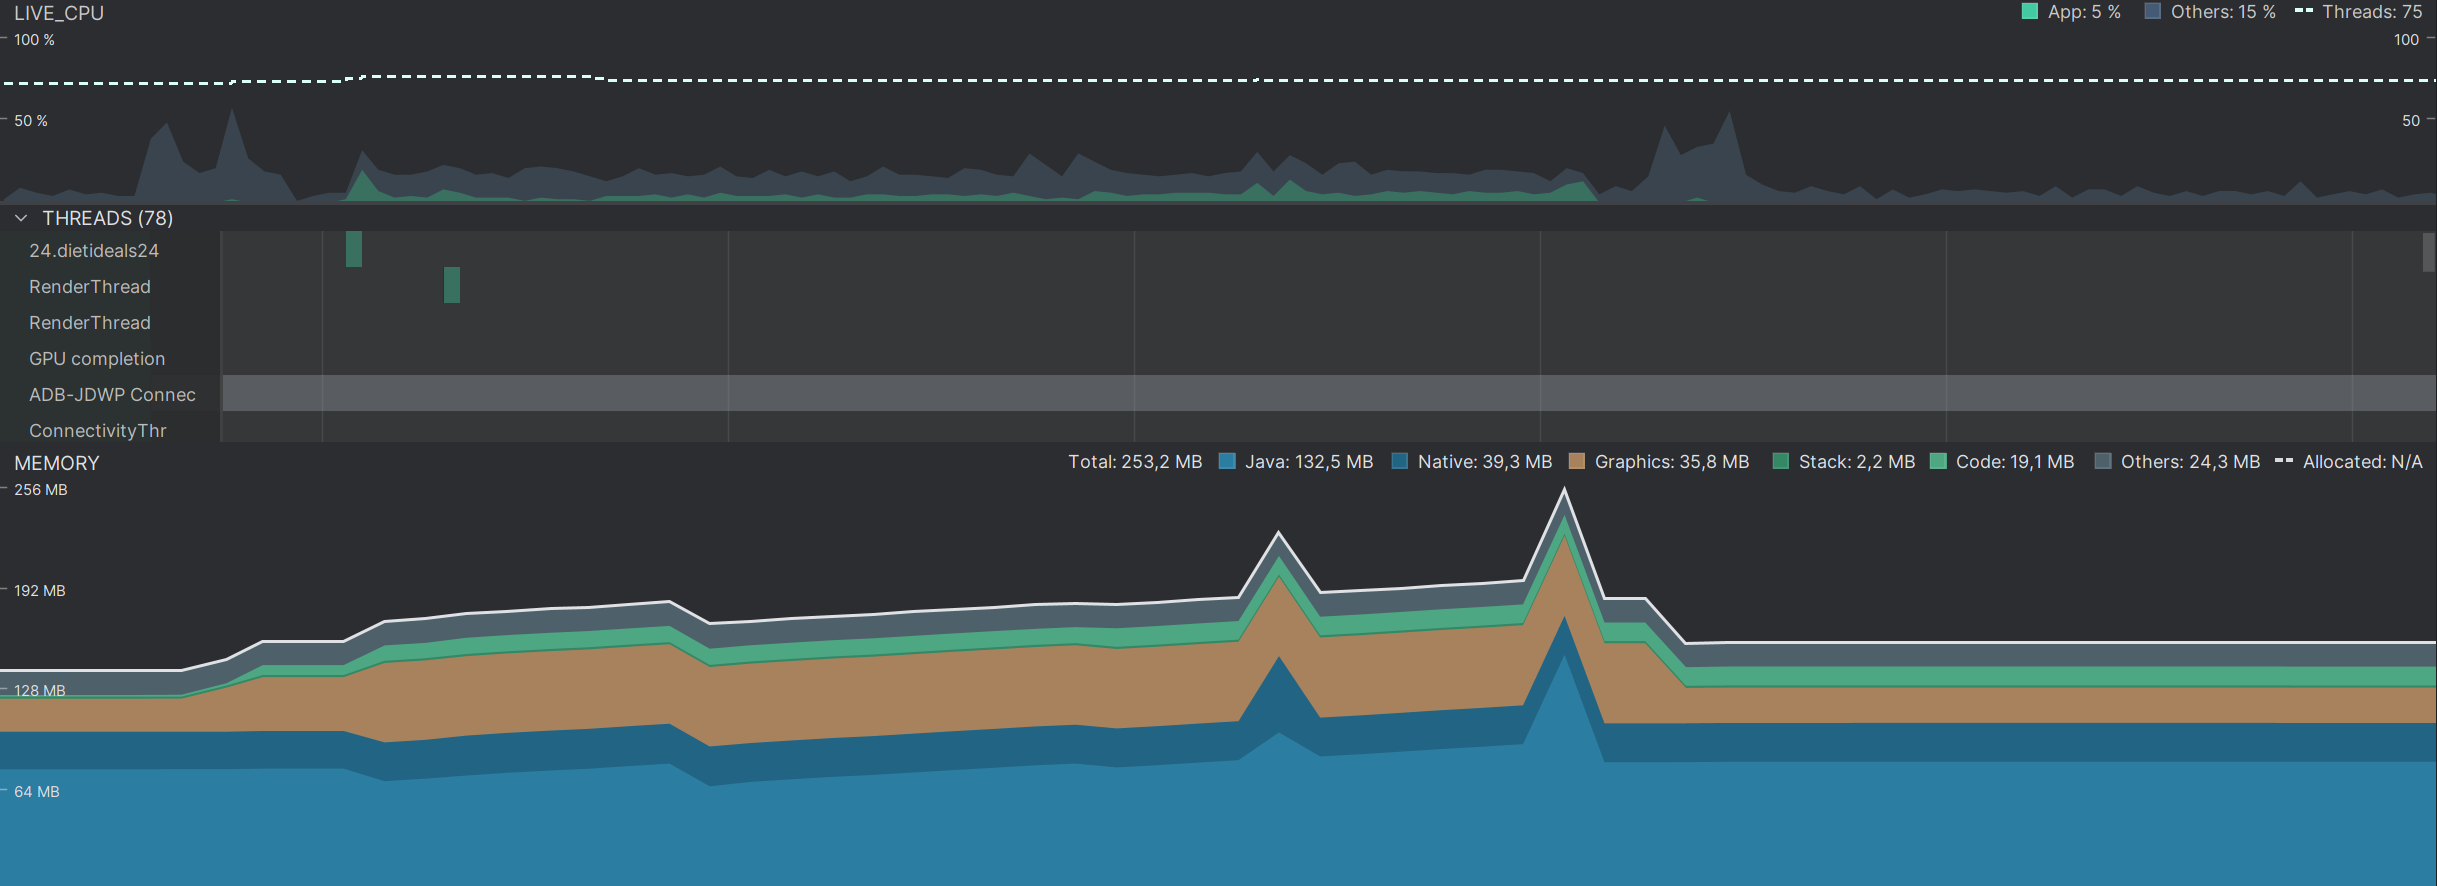
\includegraphics[width=1\linewidth]{Immagini/Validazione Software/Prestazioni.png}
            \caption{Utilizzo delle risorse dell'applicazione su client}
        \end{figure}
        Come si può osservare dal seguente grafico, estratto dal Profiler di Android Studio, le prestazioni dell'applicazione sono modeste. \\
        In circa 30 secondi di prova, consistente nello spostamento consecutivo su più schermate con relative chiamate API da effettuare ed elaborare, l'applicazione ha occupato nel punto più concitato - ossia il recupero delle aste e delle notifiche - 253,2 MB della memoria del dispositivo, come osservabile dai picchi registrati nel grafico. \\
        L'appiattimento del grafico, verso la fine, segue lo spegnimento dello schermo, confermando che l'applicazione "a riposo" consuma circa 150 MB. \\
        Come si può osservare la maggioranza della memoria è occupata dall'allocazione di classi Java, mentre le classi Kotlin native, la UI e lo stack delle chiamate si dimostrano molto più modeste. \\
        La CPU viene utilizzata appena al 5\%, mostrando che le operazioni da effettuare siano poco pesanti - a dispetto della quantità di dati da elaborare - ed adatte al tipo di dispositivo target. \\
        In quantità più elevata si possono osservare i thread generati dall'applicazione. \\
        Occorre appuntare che l'applicazione fa ampio uso dei meccanismi di Coroutines di Kotiln per scaricare il lavoro di I/O dal thread dell'interfaccia e relegarlo a thread specializzati chiamati Dispatchers, favorendo quindi la fluidità della UI e sfruttando a pieno le capacità di elaborazione concorrente dei moderni processori mobili. \\
        L'analisi non tiene conto del il calo di utilizzo che si registrerebbe quando il sistema operativo Android inserisce l'app in modalità Doze - una modalità di sonno profondo dell'app attivata dopo un lungo periodo di inutilizzo dove le operazioni vengono interrotte e solo per brevi intervalli di tempo, distanziati tra loro, all'app viene permesso effettuare operazioni in background. \\
        Si può, infine, osservare l'evoluzione dei tempi di avvio dell'applicazione Android nel corso dei precedenti 60 giorni ai test; attualmente, il valore si attesta a 789 millisecondi.
        \begin{figure}[htbp!]
            \centering
            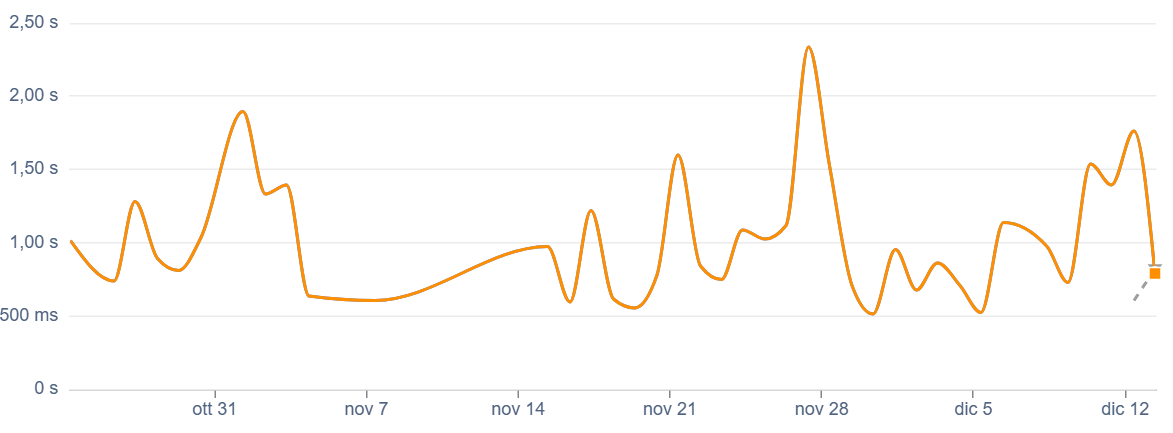
\includegraphics[width=1\linewidth]{Immagini/Validazione Software/TempoAvvio.png}
            \caption{Grafico dei tempi di avvio dell'applicazione nel corso dello scorso mese}
        \end{figure}
        
   \section{Beta test}
        Dopo aver raggiunto la maturità per una prova più estesa, l'app ha attraversato un periodo di beta test, dove è stata distribuita ad un campione ridotto di utilizzatori di sesso, età, occupazione e stato sociale differenti. \\
        Il test si è svolto lasciando libera autonomia al campione, chiedendo di utilizzare l'applicazione come farebbe normalmente se utilizzasse un'applicazione per il proprio telefono e osservando le azioni effettuate. \\
        Alla conclusione del test, è stato chiesto al campione di compilare un form per apprendere l'opinione generale e scoprire eventuali margini di miglioramento. \\
        Il form, consultabile \href{https://forms.gle/cmGryaNc8UBN3qct9}{\underline{qui}} e realizzato con Google Forms, mira a conoscere le opinioni circa la sessione di utilizzo dell'applicazione nonché esperienze pregresse con applicazioni simili. \\
        Dopo l'input delle risposte, i risultati sono stati inviati ad un file di Google Sheets collegato. \\
        Essi sono i seguenti:
        \begin{table}[ht]
            \resizebox{\textwidth}{!}{
                \begin{tabular}{l|l|l|l|l|l|l|l|l|}
                \cline{2-6}
                &
                \begin{tabular}[c]{@{}l@{}}Soddisfazione\\/10\end{tabular}\cellcolor{head} &
                \begin{tabular}[c]{@{}l@{}}Feedback\\sistema/5\end{tabular} \cellcolor{head} &
                \begin{tabular}[c]{@{}l@{}}Intuitività\\interfaccia\\/5\end{tabular}\cellcolor{head} &
                \begin{tabular}[c]{@{}l@{}}Libertà\\di\\azione/5\end{tabular}\cellcolor{head} &
                \begin{tabular}[c]{@{}l@{}}Consistenza\\stile/5\end{tabular}\cellcolor{head} &
                \begin{tabular}[c]{@{}l@{}}Prevenzione\\errori/5\end{tabular}\cellcolor{head} &
                \begin{tabular}[c]{@{}l@{}}Facilità\\di\\memorizzazione\\/5\end{tabular}\cellcolor{head} &
                \begin{tabular}[c]{@{}l@{}}Scorciatoie/5\end{tabular}\cellcolor{head} \\ \hline
                \multicolumn{1}{|l|}{Utente 1} & 8 & 3 & 3 & 2 & 2 & 2 & 3 & 3 \\ \hline
                \multicolumn{1}{|l|}{Utente 2} & 7 & 3 & 2 & 1 & 2 & 2 & 3 & 3 \\ \hline
                \multicolumn{1}{|l|}{Utente 3} & 7 & 4 & 4 & 4 & 4 & 3 & 3 & 4 \\ \hline
                \multicolumn{1}{|l|}{Utente 4} & 8 & 2 & 2 & 3 & 2 & 2 & 2 & 2 \\ \hline
                \multicolumn{1}{|l|}{Utente 5} & 6 & 2 & 2 & 3 & 3 & 3 & 2 & 3 \\ \hline
                \multicolumn{1}{|l|}{Utente 6} & 8 & 5 & 5 & 5 & 2 & 5 & 5 & 5 \\ \hline %Kevin
                \end{tabular}
            }
        \end{table}
        \begin{table}[ht]
            \resizebox{\textwidth}{!}{
                \begin{tabular}{l|l|l|l|l|l|l|l|}
                \cline{2-6}
                &
                \begin{tabular}[c]{@{}l@{}}Piacevolezza\\visiva/5\end{tabular}\cellcolor{head} &
                \begin{tabular}[c]{@{}l@{}}Facilità\\di\\comprensione\\errori/5\end{tabular}\cellcolor{head} &
                \begin{tabular}[c]{@{}l@{}}Aiuti\\e\\documentazione/5\end{tabular} \cellcolor{head} &
                \begin{tabular}[c]{@{}l@{}}Familiarità\\con la\\tecnologia\\/10\end{tabular}\cellcolor{head} &
                \begin{tabular}[c]{@{}l@{}}Già\\usato\\app\\simili\end{tabular}\cellcolor{head} &
                \begin{tabular}[c]{@{}l@{}}App\\usate\end{tabular}\cellcolor{head} \\ \hline
                \multicolumn{1}{|l|}{Utente 1} & 3 & 1 & 3 & 10 & Sì & eBay \\ \hline
                \multicolumn{1}{|l|}{Utente 2} & 2 & 2 & 3 & 4 & No & \\ \hline
                \multicolumn{1}{|l|}{Utente 3} & 4 & 3 & 3 & 8 & Sì & Amazon, Vinted, Temu \\ \hline
                \multicolumn{1}{|l|}{Utente 4} & 3 & 3 & 3 & 9 & Sì & Amazon, eBay, Subito \\ \hline
                \multicolumn{1}{|l|}{Utente 5} & 2 & 2 & 2 & 7 & No & \\ \hline
                \multicolumn{1}{|l|}{Utente 6} & 3 & 5 & 5 & 7 & Sì & Vinted, eBay, Subito \\ \hline
                \end{tabular}
            }
        \end{table}
        I punteggi in percentuale di apprezzamento delle seguenti caratteristiche (che ricalcano le euristiche di Nielsen) scaturiti dal form sono:
        \begin{itemize}
            \item Soddisfazione: $\frac{44}{60} = 0,73... = 73\%$
            \item Feedback sistema: $\frac{19}{30} = 0,63 = 63\%$
            \item Intuitività interfaccia: $\frac{18}{30} = 0,6 = 60\%$
            \item Libertà di azione: $\frac{18}{30} = 0,6 = 60\%$
            \item Consistenza stile: $\frac{15}{30} = 0,5 = 50\%$
            \item Prevenzione errori: $\frac{17}{30} = 0,56... = 57\%$
            \item Facilità di memorizzazione: $\frac{18}{30} = 0,6 = 60\%$
            \item Scorciatoie: $\frac{20}{30} = 0,66... = 67\%$
            \item Piacevolezza visiva: $\frac{17}{30} = 0,56... = 57\%$
            \item Facilità di comprensione errori: $\frac{16}{30} = 0,53... = 53\%$
            \item Aiuti e documentazione: $\frac{19}{30} = 0,63 = 63\%$
        \end{itemize}

   \section{Firebase Analytics}
        Grazie all'integrazione del frontend Android con Firebase Analytics, un servizio fornito da Google utilizzabile per ottenere delle metriche circa l'utilizzo e l'andamento dell'applicazione, si possono ricavare i seguenti dati:
        \begin{figure}[htbp!]
            \centering
            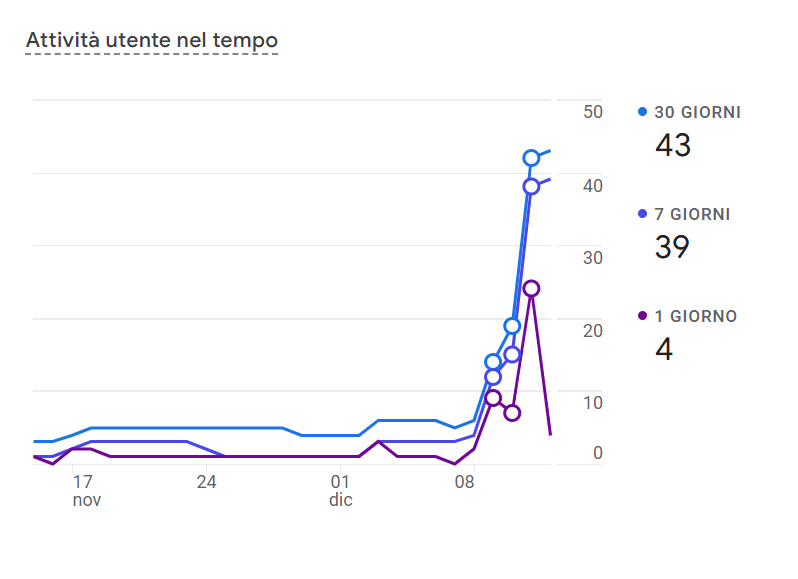
\includegraphics[width=0.5\linewidth]{Immagini/Validazione Software/UtentiAttivi.png}
            \caption{Grafico degli utenti attivi nel corso del tempo}
        \end{figure}
        \begin{figure}[htbp!]
            \centering
            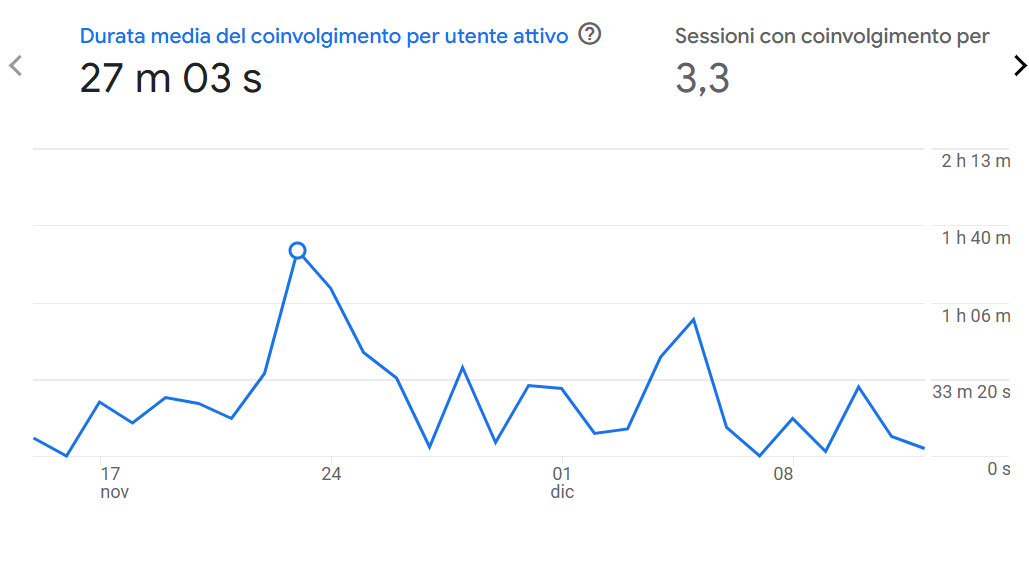
\includegraphics[width=0.5\linewidth]{Immagini/Validazione Software/CoinvolgimentoUtenti.png}
            \caption{Grafico del tempo di attività medio degli utenti}
        \end{figure}
        \begin{figure}[htbp!]
            \centering
            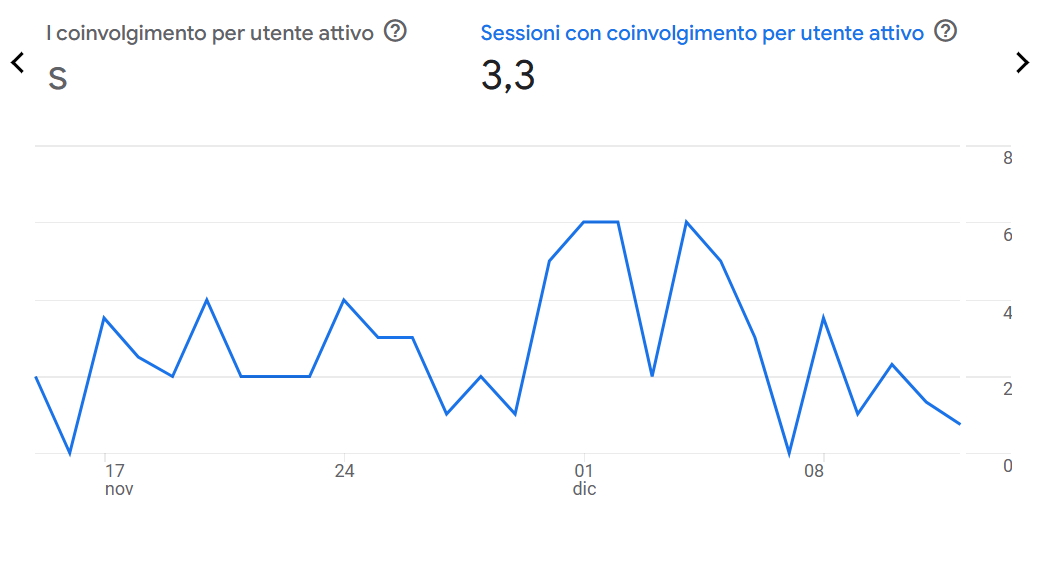
\includegraphics[width=0.5\linewidth]{Immagini/Validazione Software/SessioniUtenti.png}
            \caption{Grafico del numero di sessioni medio per ogni utente}
        \end{figure}